\documentclass{article}
\usepackage{pgfplots}
\usepackage{filecontents}
\usepackage{tikz}
\usepackage{verbatim}
\pgfplotsset{compat=1.8}
\usepackage{pgfplotstable}
\usepackage{tikz-qtree}
\usepackage{tikz-dependency}
\tikzstyle{vertex}=[draw,fill=white!15,circle,minimum size=20pt,inner sep=1pt]

\begin{document}

%% \begin{tikzpicture}
%%   \Tree [.S [.NP LaTeX ] [.VP [.V is ] [.NP fun ] ] ]
%% \end{tikzpicture}

%% \begin{dependency}
%%   \begin{deptext}[column sep=1em]
%%     A \& hearing \& is \& scheduled \& on \& the \& issue \& today \& . \\
%%   \end{deptext}
%%   \deproot{3}{ROOT}
%%   \depedge{2}{1}{ATT}
%%   \depedge[edge start x offset=-6pt]{2}{5}{ATT}
%%   \depedge{3}{2}{SBJ}
%%   \depedge{3}{9}{PU}
%%   \depedge{3}{4}{VC}
%%   \depedge{4}{8}{TMP}
%%   \depedge{5}{7}{PC}
%%   \depedge[arc angle=50]{7}{6}{ATT}
%% \end{dependency}

%% \begin{tikzpicture}[font=\sffamily,thick,level/.style={sibling distance=50mm/#1}]
%%   \node[vertex] {S}
%%   child {
%%     node[vertex] {A}
%%     child {
%%       node[vertex] {a}
%%     }
%%     child {
%%       node[vertex] {A}
%%       child { node[vertex] {a} }
%%       child {
%%         node[vertex] {A}
%%         child { node[vertex] {$\varepsilon$} }
%%       }
%%     }
%%   } child {
%%     node[vertex] {B}
%%     child { node[vertex] {b} }
%%   }
%%   ;
%% \end{tikzpicture}


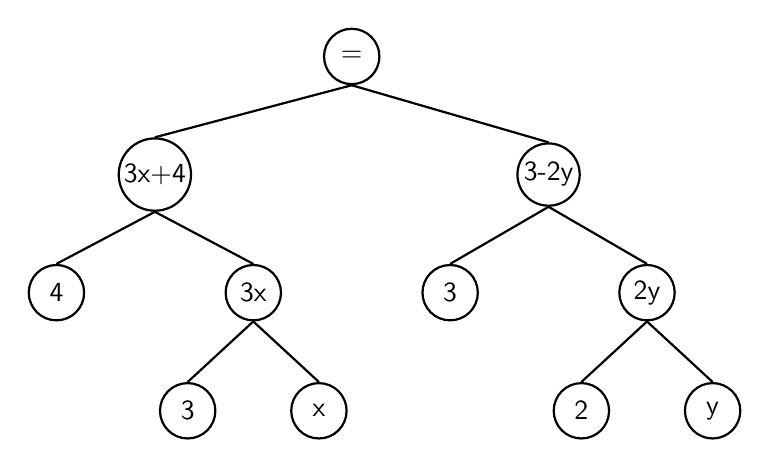
\begin{tikzpicture}[font=\sffamily,thick,level/.style={sibling distance=50mm/#1}]
  \node[vertex] {=}
  child {
    node[vertex] {3x+4}
    child {
      node[vertex] {4}
    }
    child {
      node[vertex] {3x}
      child { node[vertex] {3} }
      child {
        node[vertex] {x}
      }
    }
  } child {
    node[vertex] {3-2y}
    child {
      node[vertex] {3}
    }
    child {
      node[vertex] {2y}
      child{ node[vertex] {2} }
      child{ node[vertex] {y} }
    }
  }
  ;
\end{tikzpicture}


\end{document}
